\section{Distribution-Head Ablation Details}
\label{supp:distribution}
The ablation retains Gaussian, Laplace, fixed-$\df$ \StudentT{}, and learned-$\df$ \StudentT{} results. The learned variant is visible even though it is not the final method.
\begin{figure}[ht]\centering
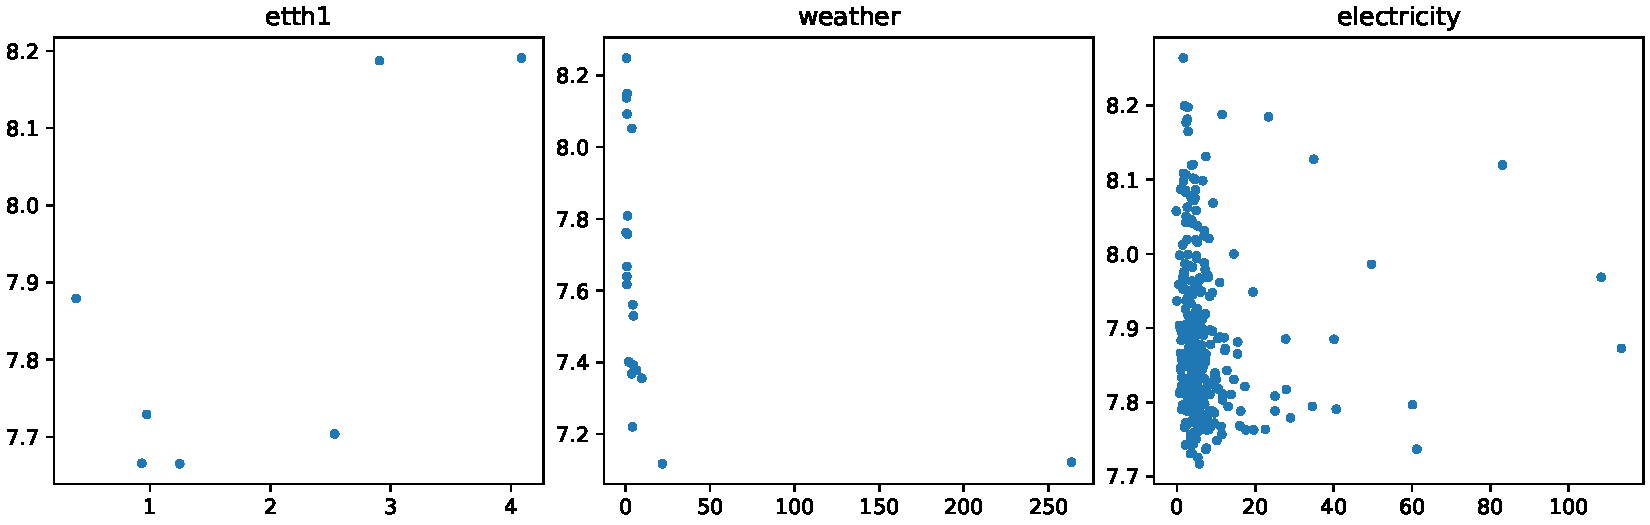
\includegraphics[width=0.48\linewidth]{fig_gate5a_kurtosis_df.pdf}
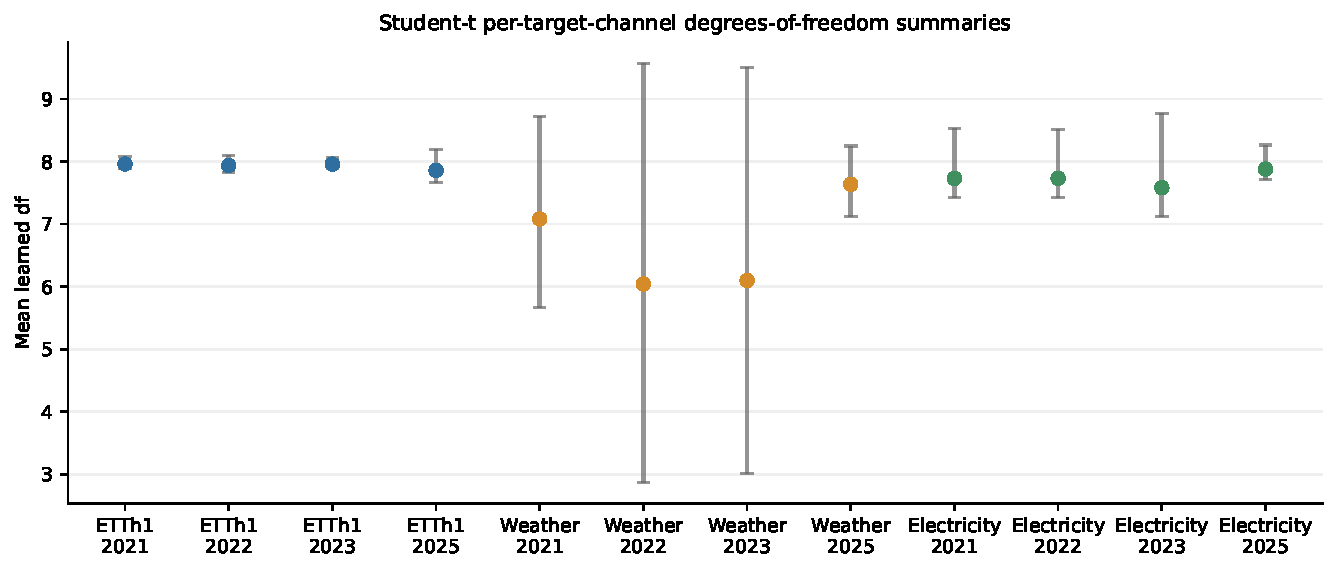
\includegraphics[width=0.48\linewidth]{fig4_student_t_df.pdf}
\caption{Descriptive channel-tail diagnostics and distribution-head comparison.}\label{fig:supp-df}
\end{figure}

\section{PIT and QQ Diagnostics}
\label{supp:pit-qq}
These probability integral transform and quantile plots are descriptive diagnostics; they are not formal evidence of joint calibration.
\begin{figure}[ht]\centering
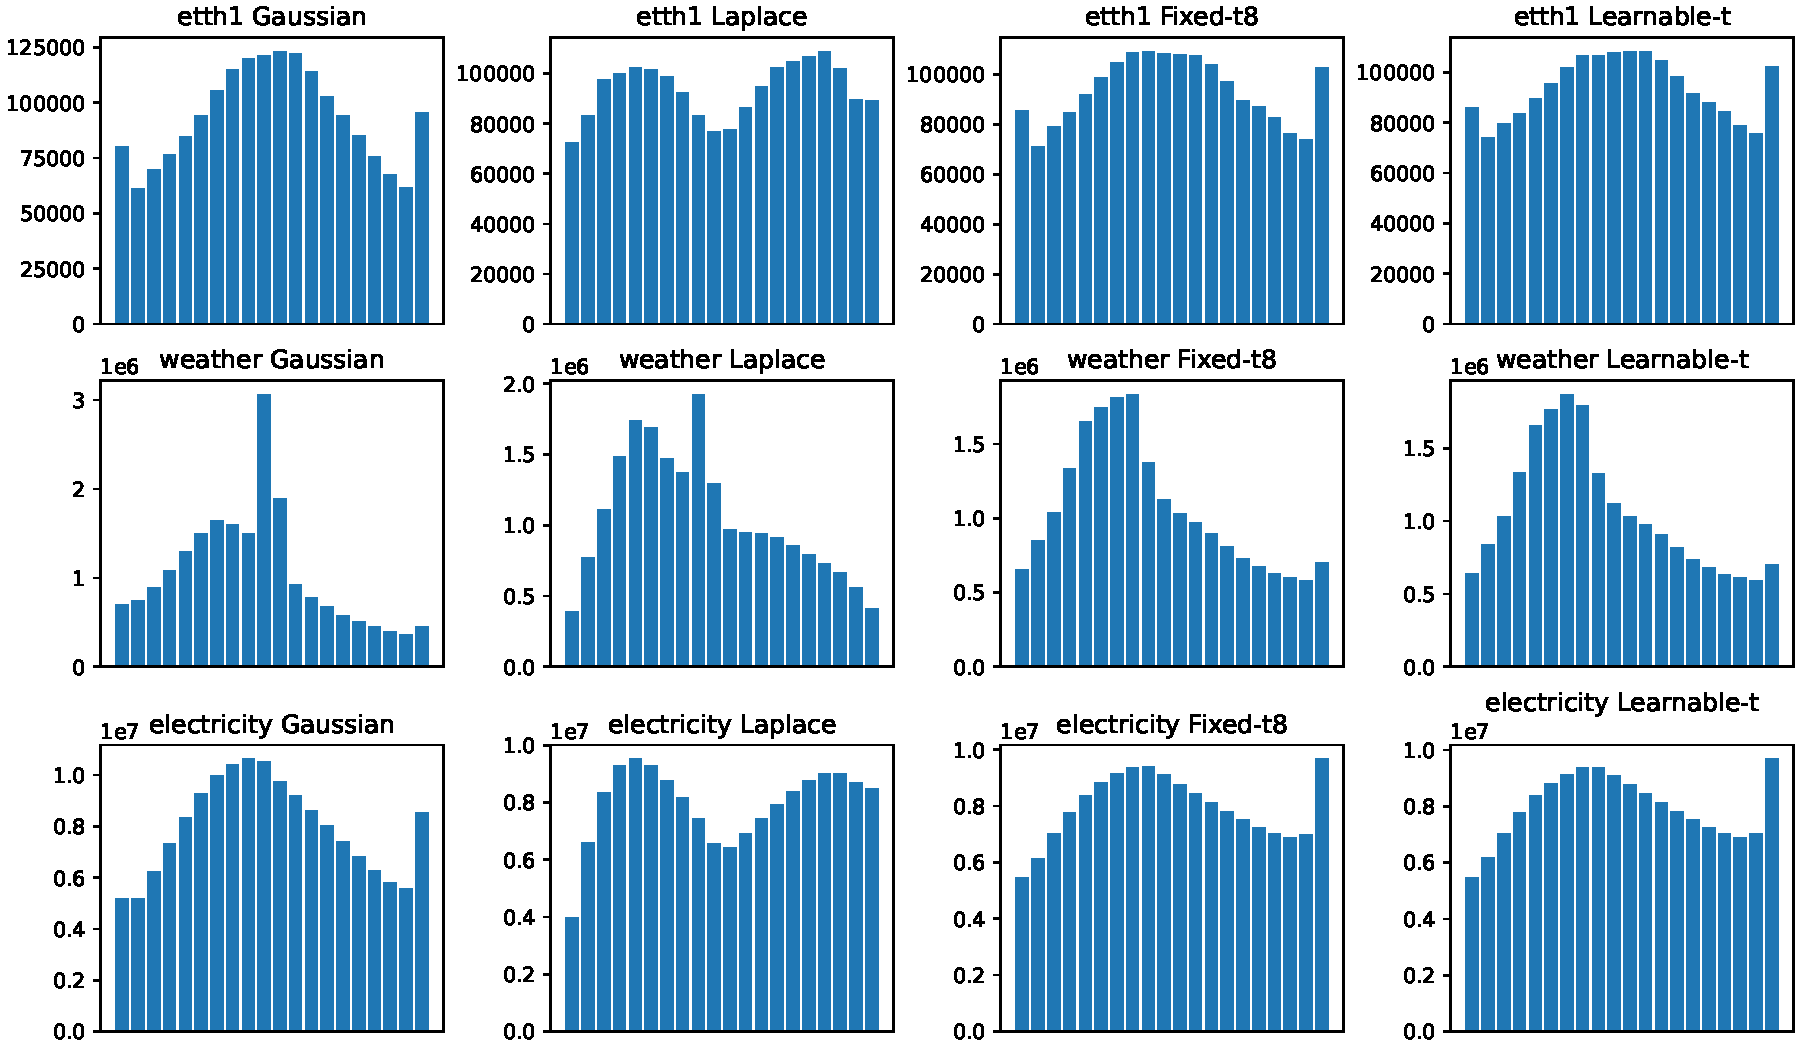
\includegraphics[width=0.48\linewidth]{fig_gate5a_pit_histograms.pdf}
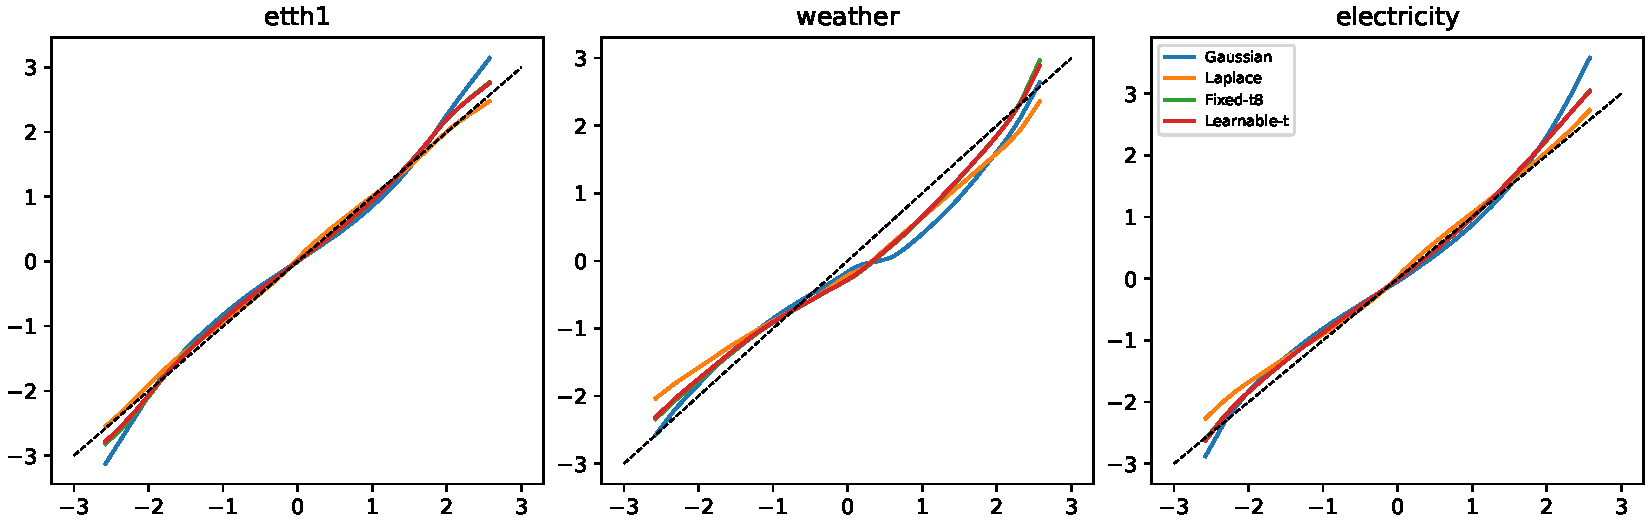
\includegraphics[width=0.48\linewidth]{fig_gate5a_qq.pdf}
\caption{PIT histograms and quantile diagnostics for the distribution ablation.}\label{fig:supp-pit-qq}
\end{figure}

\section{PatchTST Detailed Results}
\label{supp:patchtst}
The second-backbone study uses one backbone seed and one probability-head seed per dataset. ETTh1 and Weather pass the full paired criteria; Electricity preserves NLL and CRPS improvements but exceeds the 1\% point-error tolerance.
\begin{figure}[ht]\centering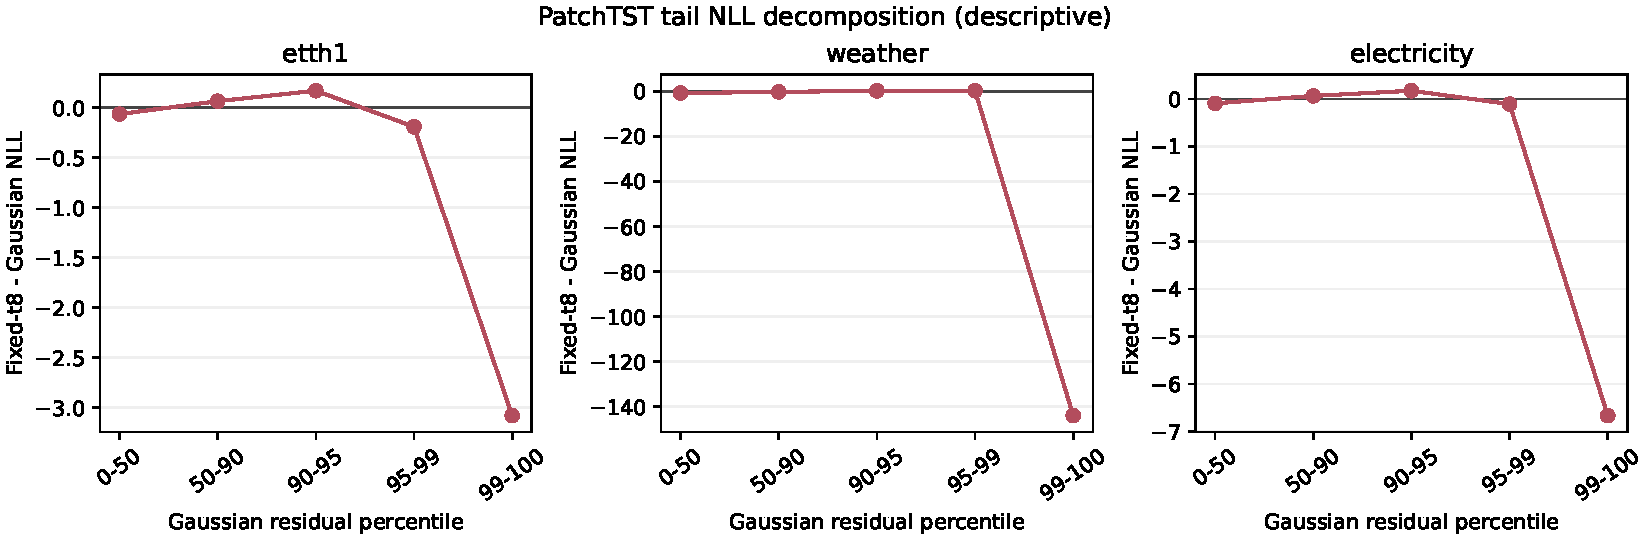
\includegraphics[width=0.82\linewidth]{fig_gate5b_patchtst_tail_nll_gain.pdf}\caption{Descriptive PatchTST tail-bin NLL decomposition.}\label{fig:supp-patchtst-tail}\end{figure}
